
\begin{figure*}[!t]

\begin{changed}
\hspace{-15mm}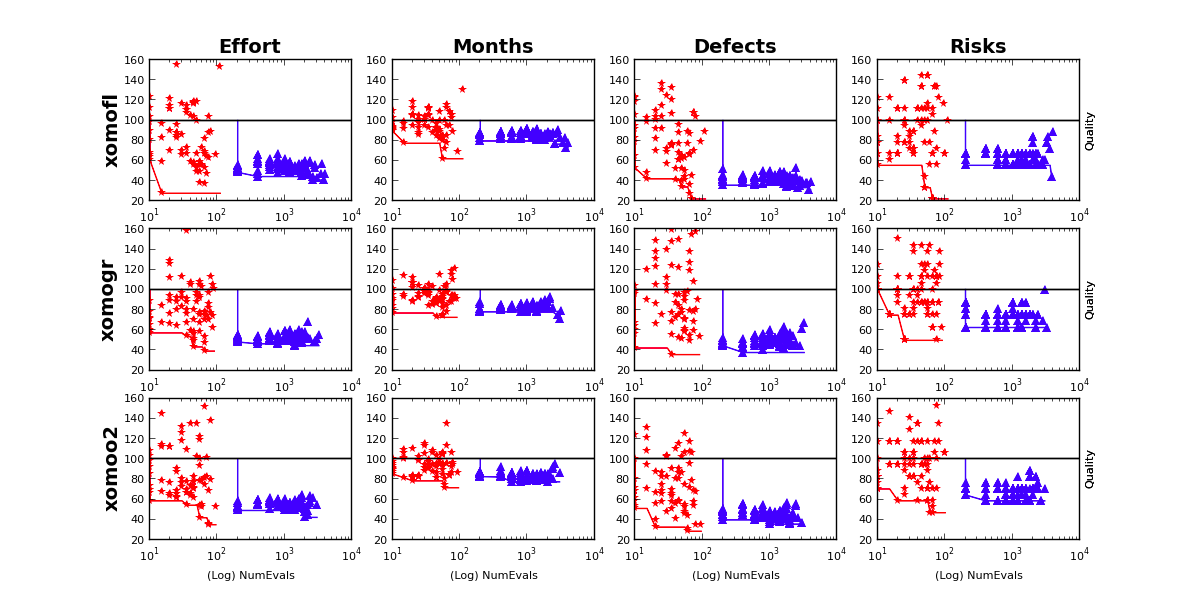
\includegraphics[width=8.5in]{figures/xomoresults.png}
\caption{XOMO results: 20 repeats of each MOEA (one row
per scenario) from
\textcolor{red}{{\bf GALE (red)}}
and 
 \textcolor{blue}{{\bf NSGA-II (blue)}}. Each y-axis represents the percent objective value relative
to that in the initial baseline population, and lower is better.
The lines trend across the best (lowest) seen objective thus far.  Each x-axis shows number of evaluations (log scale). }
\label{fig:xomoresults}
\end{changed}
\end{figure*}
